Im Februar 1969 genehmigte die NASA ( National Aeronautics and Space
Administration) ein Programm, um den Asteroidengürtel, das
interplanetare Medium zwischen Mars und Jupiter, die äußeren Planeten
und Fly-By Manöver zu erforschen. Hierzu wurden zwei baugleiche Sonden
Pioneer F (Pioneer 10 Mission) und Pioneer G (Pioneer 11 Mission) zum
Jupiter gebracht. Die Pioneer 10 Mission startete am 2. März 1972 und
wurde dann auf ca. 14,4 km/s beschleunigt. Die Sonde durchflog im Juli
1972 unbeschadet den Asteroidengürtel und erreichte am 4. Dezember 1973
den Jupiter. Hier nutzte man ein Fly-By Manöver um die Sonde auf eine
heliozentrische Fluchtgeschwindigkeit von 11,322 km/s
(Gesamtgeschwindigkeit 36,7 km/s)zu beschleunigen um das Sonnensystem
in Richtung des Sterns Aldebaran (Laut Zeitplan sollte die Sonde den
Stern in ungefähr 2 Millionen Jahren erreichen\cite{Nieto2007}) zu verlassen.
Pioneer 11 startete
13 Monate später, am 6. April 1973, da die NASA mit Pioneer 10 erst
herausfinden wollte, ob eine Durchquerung des Asteroidengürtels
überhaupt möglich ist. Ihre Bahn führte Pioneer 11 ebenfals Richtung
Jupiter, den sie am 2. Dezember 1974 erreichte. Das dort durchgeführte
Fly-By Manöver brachte sie auf eine Bahn, die Pioneer 11 zunächst
wieder innerhalb der Jupiter-Bahn führte, um dann aber am 1. September
1979 den Saturn zu erreichen (Abb. \$1) In einem weiteren Fly-By
Manöver, bei dem die Sonde die Ringe des Saturns unbeschadet durchquert
hat, wurde sie auf eine asymptotische Fluchtgeschwindigkeit von 10,450
km/s gebracht. Pioneer 11 steuert auf die Konstellation Aquila zu, wo
sie in ungefähr 4 Millionen Jahren eintreffen wird. Die Relationen der
Flugbahnen der Sonden Pioneer 10 und 11, sowie Voyager 1 und 2 sind in
Abb. \$2 zu erkennen.


\bigskip

Abb. \$1 und \$2

%\begin{minipage}[hbt]{6cm}
%	\centering
%	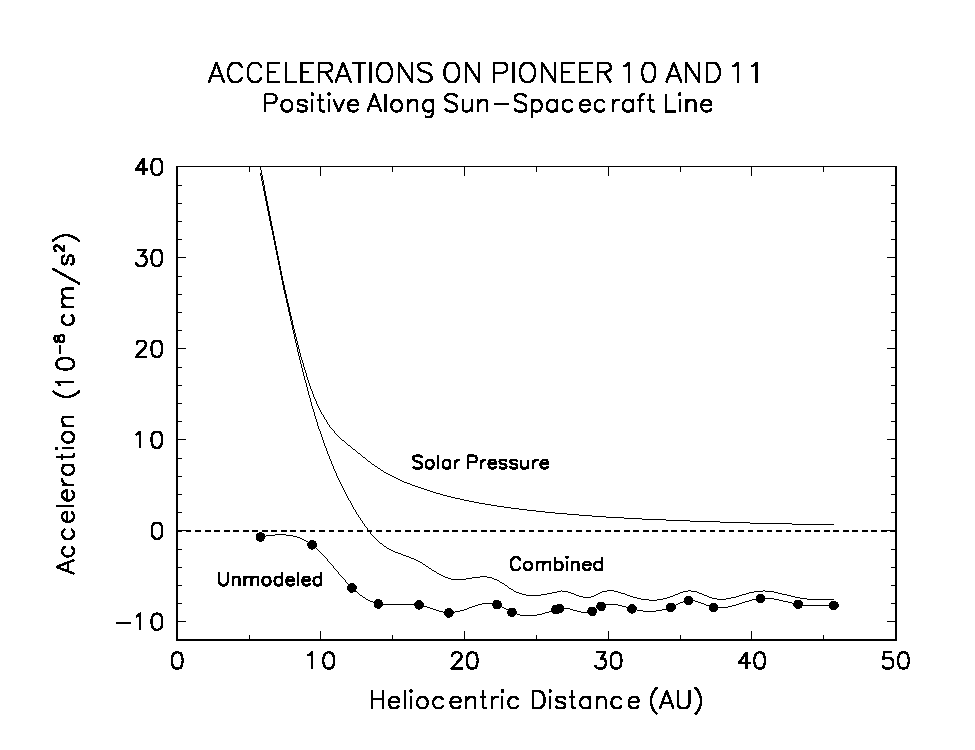
\includegraphics[width=6cm]{cOMBINED}
%	\label{Bild1}
%\end{minipage}
%\hfill
%\begin{minipage}[hbt]{6cm}
%	\centering
%	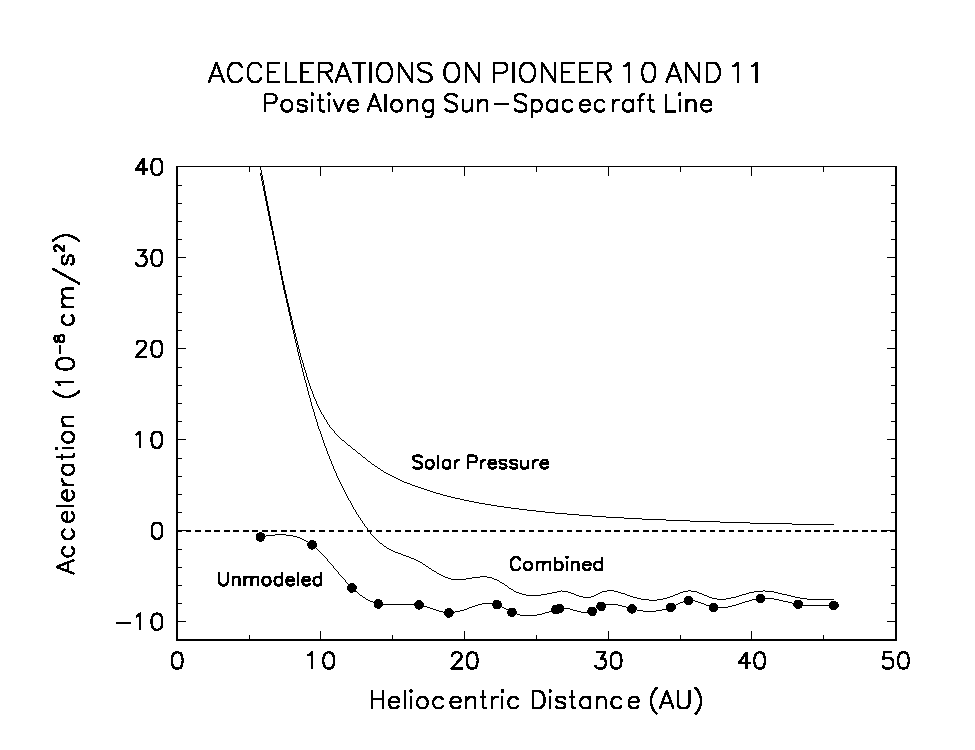
\includegraphics[width=6cm]{cOMBINED}
%	\label{Bild2}
%\end{minipage}

\bigskip

Obwohl Pioneer 10 und 11 nur auf eine Betriebszeit von 21 Monate
ausgelegt waren, sendete Pioneer 10 Messdaten bis zum 27. April 2002.
Das letzte Signal von Pioneer 10 erreichte die Erde am 23. Januar 2003.
Das letzte Signal von Pioneer 11 wurde jedoch deutlich früher, am 24.
November 1995 empfangen, da durch das zweite Fly-By Manöver am Saturn
sehr viel mehr Leistung benötigt wurde.
Zu den o.g. Missionszielen gehörte vor allem unter dem Punkte der
Erforschung der äußeren Planeten die Suche nach dem „Planeten X“, der
damals jenseits von Neptun vermutet wurde. Um das schwache
Gravitationsfeld dieses ominösen Planeten nachzuweisen und um möglichst
nahe an Jupiter und Saturn vorbei zu fliegen, benötigten die
Pioneer-Sonden eine sehr genaue Navigation. Dabei wurden von einer
Bodenstation des Deep Space Network DSN (in Goldstone/USA,
Madrid/Spanien, Canberra/Australien) Radiowellen mit einer
wohldefinierten Frequenz zur Sonde geschickt. Die Pioneers sendete
dieses Signal mit einer um den Faktor 240/221 konvertierten Frequenz
wieder zur Erde zurück\cite{Dittus2006}. Diese genaue
Navigation erlaubte schließlich die Entdeckung der Pioneer-Anomalie. 
Damit die Parabolantenne immer auf die Erde gerichtet blieb, musste
die Sonde vor allem nach Vorbeiflügen an großen Planeten neu
ausgerichtet werden. Hierzu wurden kleine Triebwerke für eine kurze
Zeit gezündet. Alle weiteren Störfaktoren auf die Flugbahn von Pioneer
10 und 11 wurden mit einer Eigenrotation der Sonden um die
Symmetrieachse der Parabolantenne von 4 bis 7 U/min
ausgeglichen\cite{Dittus2006}\cite{Nieto2007}.
Durch die genaue Navigation und die Verminderung von Fehlern,
bemerkte man Anfang der 80er eine unvorhergesehene Beschleunigung von
$(8,74+-1,33)*10^{-8} cm/s^{2}$ \cite{Anderson2002} in Richtung der Sonne. 

Diese Beschleunigung wurde schließlich zur Pioneer-Anomalie, deren
Ursache bis heute nicht bekannt ist.
